\chapter{Physical problems addressed in this thesis} 
%
\InitialCharacter{T}he physical problems addressed in this thesis are introduced in this chapter. 
First, the dark matter (DM) observed in the Universe and the features that support its presence are explained. 
Also, the gamma-ray excess found in the galactic center of the Milky Way Galaxy is discussed in the context of the possible observation of DM annihilation. 
At the end, the chapter is focused in the neutrino masses and the possible relation between the DM and neutrino physics at one-loop level.  










\section{The dark matter in the Universe}
\label{sec:intro-dark-matter}
%
It is well established that the DM makes up about $26\%$ of the energy density of the Universe. It is about six times more abundant than ordinary matter~\cite{Ade:2015xua}.
However, its fundamental nature remains mysterious.
There is not known particle with the properties needed to constitute the DM, whose identity begs for new physics beyond the standard model (SM).
Unveiling which particle accounts for the majority of the matter in the Universe is a key open question at the interface of particle physics and cosmology.

Promising candidates for DM particles are weakly interacting massive particles (WIMPs).
These are generally assumed to be at equilibrium in the early Universe, but then freeze-out due to the rapid expansion of the Universe.
If the WIMP masses are in the GeV to TeV range, and the annihilation cross sections are of order the weak interaction scale, the relic DM density measured by experiments today arises naturally~\cite{Kolb:1990vq}.
% * <restrepo@udea.edu.co> 2016-09-21T12:20:31.236Z:
% 
% Esto ya no es del todo cierto. En esa época se referían a la mediación 
% con el Z que ya esta descartada.  Ver las slides de la charla de Oscar en Ibague, slide 16: 
% https://goo.gl/1s9QH8
% 
% ^. --> Falta (Andrés)
In general, there are some experimental facts that support the DM idea and therefore the structure formation in the Universe~\cite{Kolb:1990vq}. 
Some of them are shown in Fig.~\ref{fig:evidences} and they will be briefly discussed in the following. 
%
\begin{figure}[h]
\centering
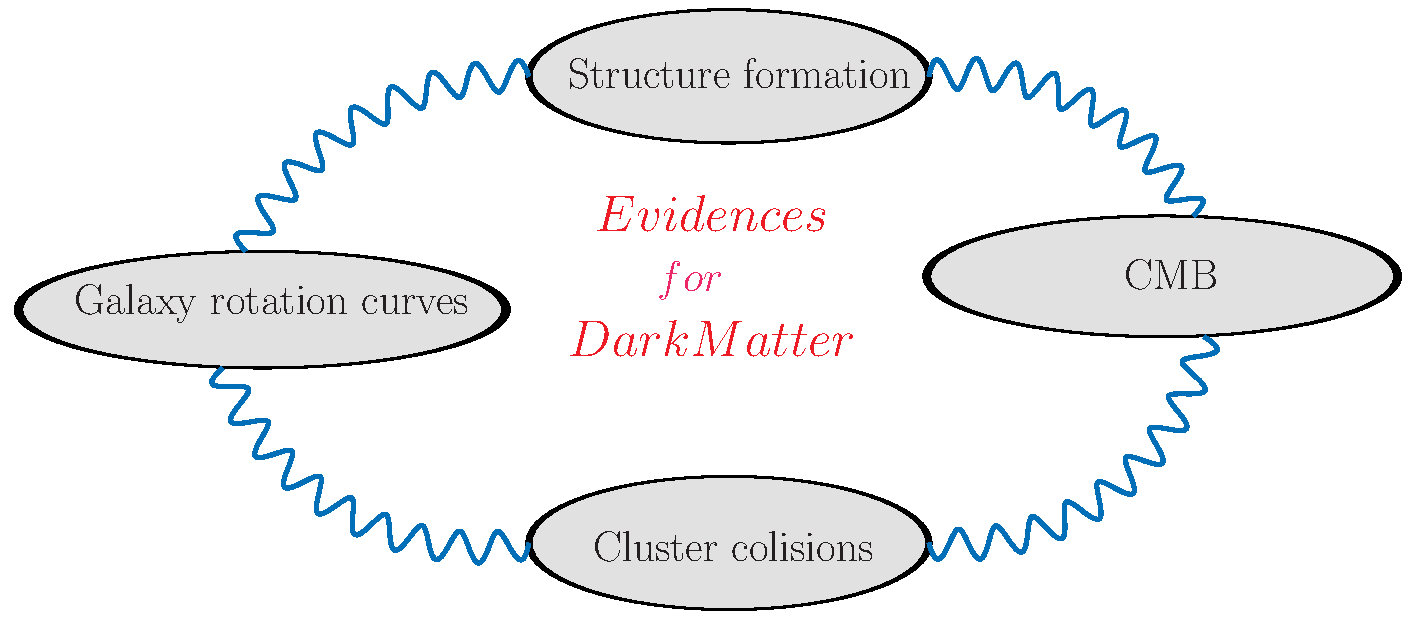
\includegraphics[width=10 cm, height=5.0 cm]{fig3.pdf}
\caption{Some of the most important evidences for Dark Matter.}
\label{fig:evidences}
\end{figure}










\begin{itemize}
\item[i.] \textbf{Galaxy rotation curves}

The rotation curve of a Galaxy (cluster) is the profile of the circular velocity
of the stars (galaxies) around the mass center of the system. 
It plays an important role because it is possible
to infer the mass distribution of the Galaxy (cluster)  after the analysis of this profile. 
Historically, the relation between the mass distribution and the rotation curve was first proposed by Fritz Zwicky in 1937.
He analyzed the velocity dispersion of the galaxies in the Coma cluster, assuming that the outer galaxies were in circular motion around its mass center.
He applied the virial theorem to the Coma cluster in order to estimate its mass and found that roughly 800 galaxies should  exhibit velocities of 80 km/h, however, the observed velocity dispersion was approximately 1000 km/h~\cite{1937ApJ-86-217Z}. 
The problem was known as the \textbf{Galaxy rotation problem} (for a complete historical discussion see the Ref.~\cite{Bertone:2016nfn}). 
%
\begin{figure}[h]
\begin{center}
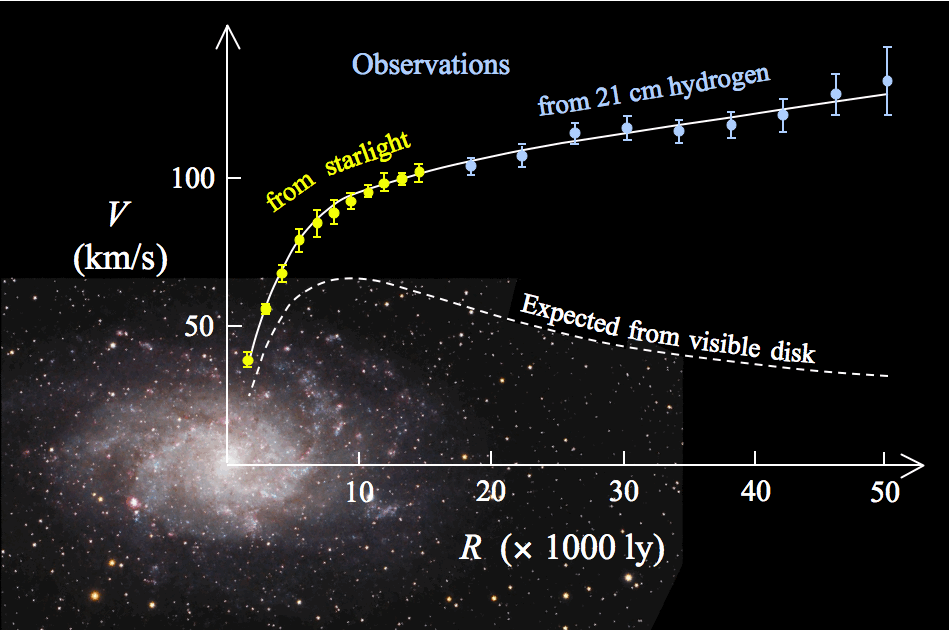
\includegraphics[scale=0.35]{M33_rotation_curve_HI}
\end{center}
\caption{Rotation curve of the typical spiral Galaxy M 33 (yellow and blue points with errorbars) and the predicted one from the distribution of the visible matter (white dashed line). The best fit model for rotation curve is represented by the continuous white line ~\cite{Corbelli:1999af} (Taken from Wikipedia - Public Domain).}
\label{fig:M33}
\end{figure}
%
The general idea under this problem is that when the Newton mechanics is used to explain the velocity distribution of the stars and visible gas in a Galaxy, the obtained profile (dashed white line in Fig.~\ref{fig:M33}) does not match with the observed behavior that is measured with some astrophysical techniques such as mass-to-light ratio~\footnote{The mass-to-light ratio ($\Upsilon$) is the relation between the total mass of a Galaxy and its luminosity. In astrophysics the reference value is the mass-to-light ratio of the sun, for that reason for big objects dominated by DM have a big mass-to-light ratio.} and the distribution of stars in the spiral galaxies.  
This problem is solved if the existence of dark hidden mass is supposed (dark, because it does not have electromagnetic interactions). Dark hidden mass is present in the Galaxy with a special distribution which governs its gravitational behavior, giving the characteristical name of \textit{dark matter} (DM).










\item[ii.] \textbf{The cosmic microwave background (CMB) }

\begin{figure}[h]
\begin{center}
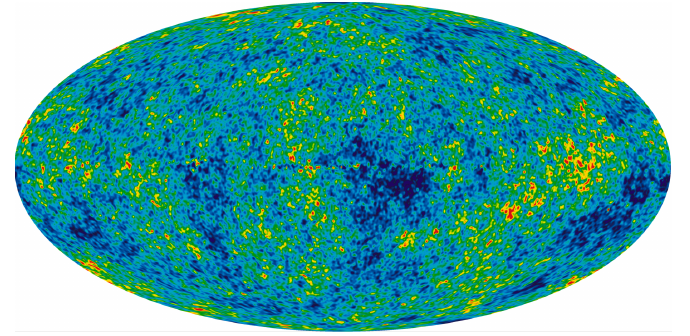
\includegraphics[scale=0.6]{CMB}
\end{center}
\caption{Nine Year Microwave Sky The detailed, all-sky picture of the infant Universe created from nine years of WMAP data. The image reveals $13.77$ billion-year-old temperature fluctuations (shown as color differences) that correspond to the seeds that grew to become the galaxies. The signal from our Galaxy was subtracted using the multi-frequency data. This image shows a temperature range of $\pm 200$ microKelvin. Credit: NASA / WMAP Science Team WMAP $\# 121238$ Image Caption $9$ year WMAP image of background cosmic radiation ($2012$).  (Taken from Wikipedia - Public Domain).}
\label{fig:CMB}
\end{figure}

The cosmic microwave background (CMB) is the oldest snapshot of the Universe that we have.
It is the thermal radiation when the Universe was approximate  $380.000$ years old after the big bang ($z\approx 1100, T\approx 3000$ K).
This radiation was generated in a time in the thermal history of the Universe called recombination or ``time of the last scattering'', which was the time when the electrons and protons formed bound states and created the neutral hydrogen in the Universe. Consequently, it was the time when the Universe began to be transparent to the photons because the atoms could not longer absorb the thermal radiation (photon decoupling). From that moment,  photons have been freely propagating.

The CMB was accidentally discovered in 1964 by the American radio astronomers Arno Penzias and Robert Wilson. For that achievement, they were awarded the Nobel Prize in 1978. This discovery was considered a big test of the big bang theory and the cosmological lambda cold dark matter model (Lambda-CDM or $\Lambda$-CDM).

In general, the CMB map shown in Fig.~\ref{fig:CMB} has a thermal black body spectrum at a temperature of $2.72548 \pm 0.00057$ K with a spectral radiance of 160.23 GHz, i.e. in the microwave range of frequencies. Even more, this spectrum  shows tiny temperature fluctuations that correspond to regions of slightly different densities that were the seeds of all the structures as the galaxies that are present in the Universe. 
%
Theoretically, those temperature fluctuations are generally expanded in the basis of spherical harmonics ($Y_{lm}$) as~\cite{Dodelson:1282338, Kolb:1990vq}
%
\begin{align}
\dfrac{\Delta T}{T}=\sum_{l,m} a_{l,m} Y_{lm}(\theta,\phi) \,,
\end{align}
%
where $\theta$ and $\phi$ are the spherical angles on the sky. Using this expansion, it follows that the two-point function of the coefficients $a_{lm}$:
%
\begin{align}
\langle a_{lm} a^*_{l^{'}m^{'}} \rangle = \dfrac{2\pi \delta_{ll^{'}}\delta_{mm^{'}}}{l(l+1)} \mathcal{D}_l \,,
\end{align}
%
determines the power spectrum of temperature $\mathcal{D}_l$ shown in Fig.~\ref{fig:T-spectrum}.
%
\begin{figure}[h]
\begin{center}
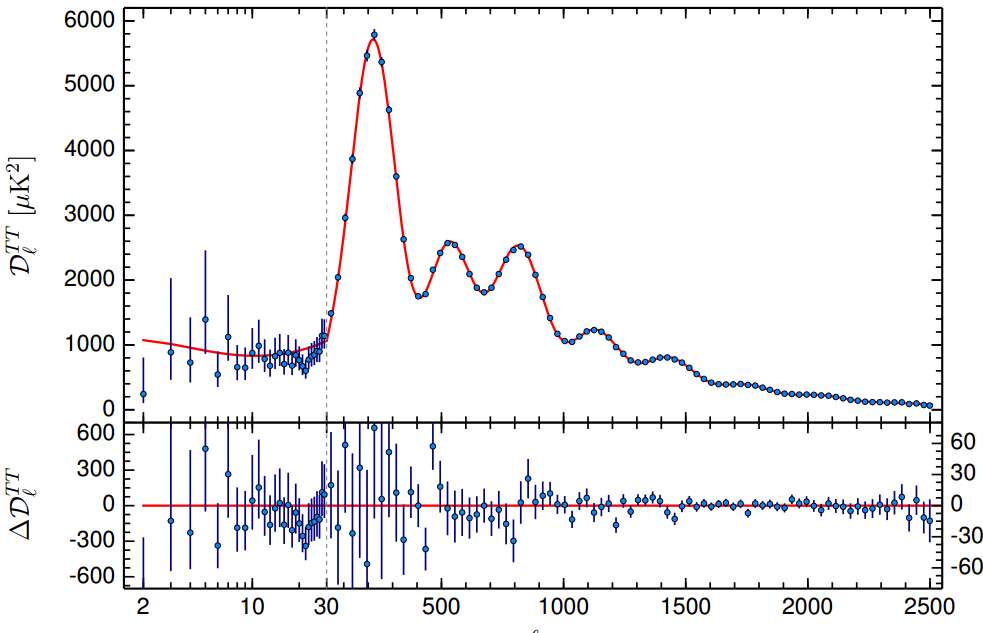
\includegraphics[scale=0.42]{spectrum}
\end{center}
\caption{Planck 2015 temperature power spectrum~\cite{Ade:2015xua}. For multipoles $l \geq 30$ is show the maximum likelihood frequency-averaged temperature spectrum. The best-fit, i.e. the $\Lambda$CDM theoretical spectrum is fitted in the upper panel. Residuals with respect to this model are shown in the lower panel. The error bars show $\pm \sigma$ uncertainties.}
\label{fig:T-spectrum}
\end{figure}

A careful analysis of the spectrum in Fig.~\ref{fig:T-spectrum} shows some special features associated with the primordial (secondary) anisotropies that occurred before (after) the photon decoupling, which are associated with the interactions of the background radiation with the hot gas and the gravitational potentials. Those anisotropies are principally determined by two effects that can be clearly seen in Fig.~\ref{fig:CMB} and Fig.~\ref{fig:T-spectrum}. Briefly, those are:
%
\begin{itemize}
\item[\textbullet ] The acoustic oscillation: In the primordial plasma there was a competition between the photons and baryons. The former tend to erase all the anisotropies and the later moving at a speed much slower than light tend to collapse to form overdensities. It is in this way that  the peaks of the CMB spectrum correspond to resonances in which the photons have decoupled from the plasma with a particular mode. 
Roughly speaking, the angular scale of the first peak in Fig.~\ref{fig:T-spectrum} with $l\approx 200$ ($\approx 1^o$ in galactic coordinates) determines the curvature of the Universe. For instance, the latest Planck data  combined with gravitational lensing and baryon acoustic oscillation (BAO)~\cite{Ade:2015xua} indicate that $\Omega_k = 0.000 \pm 0.005$ to $95\%$ confidence level. This means that the Universe is spatially flat at high precision.  
The ratio between the second and the first peak determines the baryon density. For instance, $\Omega_bh^2= 0.02230 \pm 0.00014$~\cite{Ade:2015xua}.
Finally, the third peak in combination with the first and the second peak can be used to obtain information about the dark matter density in the Universe, it is $\Omega_{\text{DM}}=(0.1197\pm 0.0022)$~\cite{Ade:2015xua}.

\item[\textbullet ] The diffusion damping: It is a physical process which reduced density inequalities (anisotropies) in the early Universe making the CMB more uniform. It happened when the photons traveled from the hot regions to the cold ones. It is important when the Boltzmann equation is computed for the CMB, which is not the scope of this work. 

\end{itemize}












\item[iii.] \textbf{Cluster collisions}

In $2006$ a group of astronomers published other direct empirical proof of the existence of the DM~\cite{Clowe:2006eq}. They studied the merging of two clusters of galaxies 1E 0657-558 ($z=0.296$) collectively known as the bullet cluster which collision is estimated that happened $\sim 100$ Mys ago and approximately in the plane determined by the velocities of the galaxies (see Fig.~\ref{fig:bullet}). 
%
In general, they found that there are two concentrations of galaxies separated by $\sim 0.72$ Mpc. The right one is moving away at $\sim 4700$ km s$^{-1}$ and it is creating a bow shock that gives its famous name of bullet cluster. 
%
\begin{figure}[h]
\centering
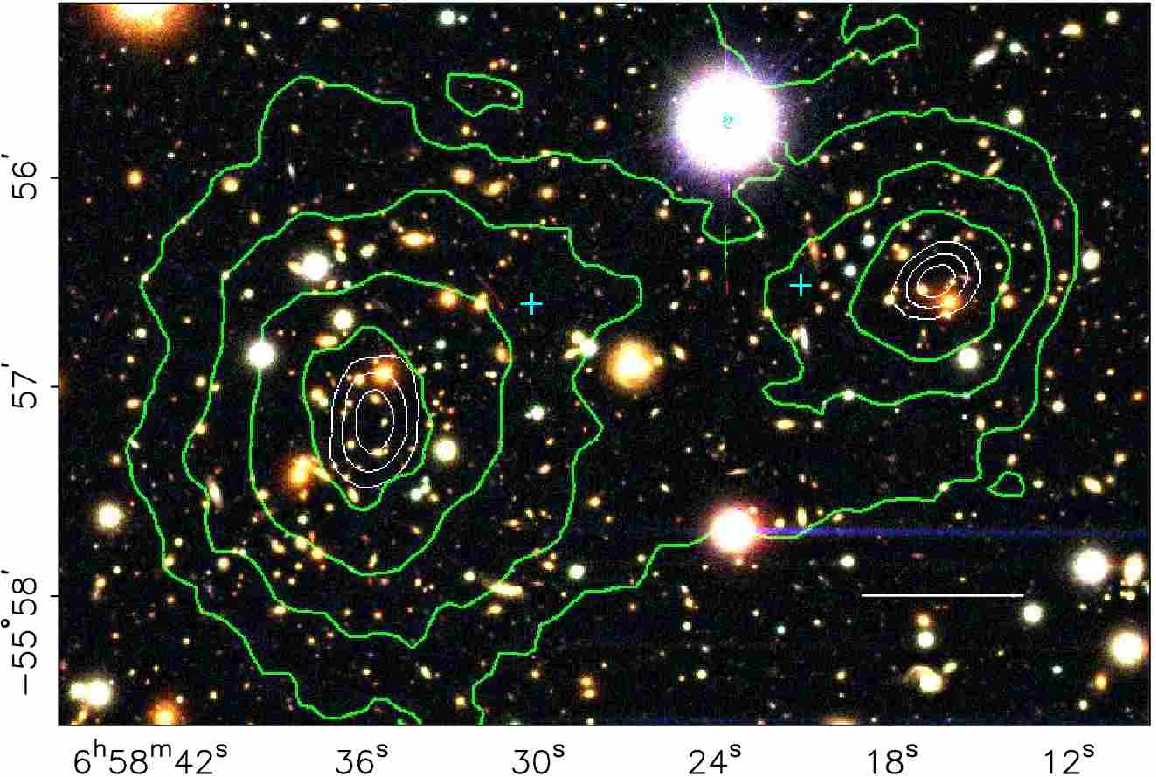
\includegraphics[scale=0.4]{bullet1}
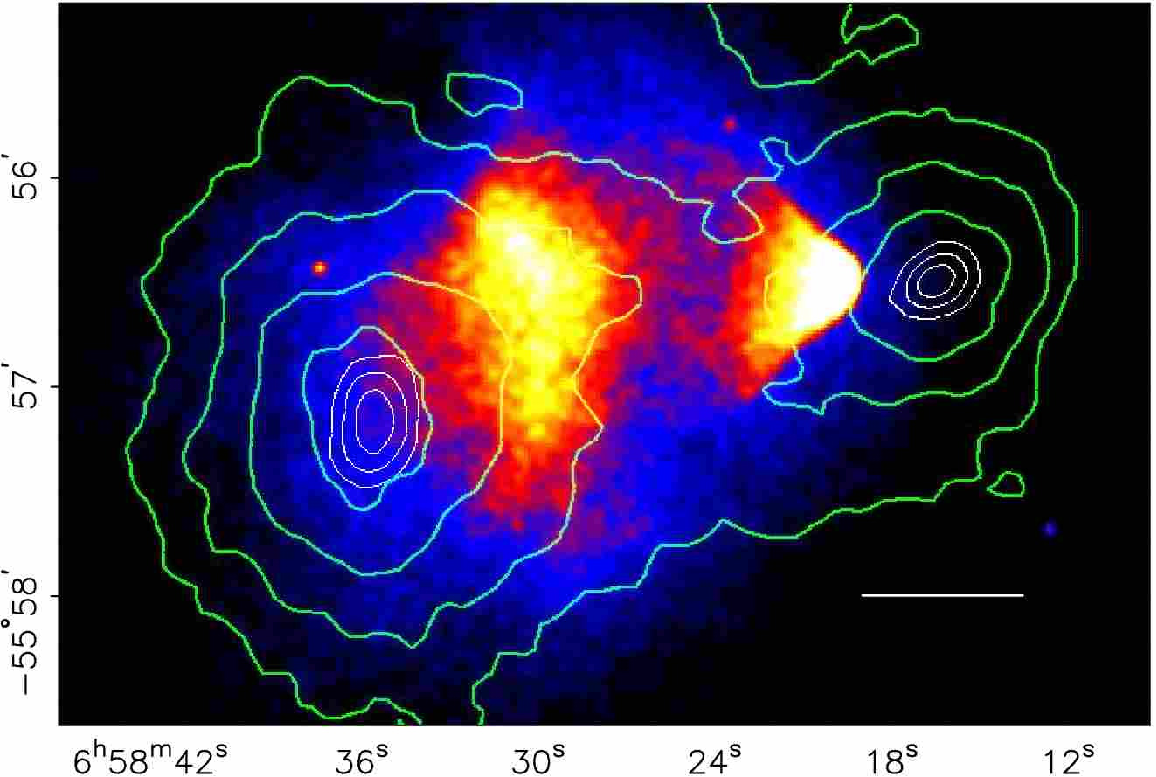
\includegraphics[scale=0.4]{bullet2}
\caption{The bullet cluster. The green contours are the reconstruction with gravitational lensing which is proportional to the mass of the system. The white bar represents a distance of $200$ kpc at the location of the cluster. The colored map on the right shows the same image seen in X-ray for the merging cluster. It was taken with the Chandra satellite after $500$ seconds of exposure. Taken from~\cite{Clowe:2006eq}.}
\label{fig:bullet}
\end{figure}
%

This observation is basically the discovery of one system in which the baryonic matter was separated from the mass center of each cluster involved in the collision. It was inferred as follows.
%
On the one hand, using gravitational lensing, the astronomers were able to reconstruct the contours of the mass projected for the system. They are represented by the green contours in Fig.~\ref{fig:bullet}. 
Basically, the gravitational lensing technique measures the distortion of the images caused by the gravitational deflection of light by the mass of the clusters and create a profile of the mass distribution inside the clusters itself. 
%
On the other hand, using the Chandra observation of X-rays they were able to see the X-rays emitted by the baryonic plasma of the system. The centers of the plasma are shown with the plus signs in the left panel of Fig.~\ref{fig:bullet}. Yellow and red parts of the image represent the baryonic plasma which emits the X-rays. Clearly, this hot plasma does not trace the mass distribution found with the gravitational lensing reconstruction. 

As a conclusion, during the merger, the galaxies behave to be almost collisionless and the hot plasma decouples of mass that is inferred by gravitational lensing. 
It can be understood if we think in two clouds of particles that are colliding. Almost all the particles pass through each other, i.e. they are collisionless and only the particles that represent the baryonic mass of the system collides.
According to this interpretation, the principal component of the mass of the system does not interact, it is dark (not baryonic) and correspond to the green contours shown in Fig.~\ref{fig:bullet}. 
%
Note that this observation is in favor of the DM interpretation as a particle. Even more, an alternative explanation using theories of Modified Newtonian Dynamics of the gravity  (MOND) does not predict an offset between mass and light and could fail to explain this observation of the bullet cluster~\cite{Angus:2006qy}.

\end{itemize}








%CONECTION
After this brief discussion of some of the facts that support the dark matter idea, it is important to describe briefly how to looking for  those  particles. 










\section{How to search for dark matter?}
\begin{itemize}

\item \textbf{Direct detection:}

The idea of direct detection of DM is based on the fact that DM particle (WIMP) is capable of collide with nucleons.
%For that reason, some experiments have been built with the purpose of collecting the signature when the DM collides with %nucleons.
%
In general, the cross section $\sigma$ for this interaction will depend on the naturalness of the DM. 
In particular, if the cross section depends of the spin of nucleons, it is called spin-dependent ($\sigma_{\text{SD}}$), otherwise,  spin-independent ($\sigma_{\text{SI}}$).
%
Until now, among the experiments for direct detection of DM, the most restrictive is the Large Underground Xenon experiment (LUX)~\footnote{\url{http://luxdarkmatter.org/}} ,
which is located 1,510 m underground at the Sanford Underground Laboratory in the Homestake Mine in Lead, South Dakota.
It is operated underground to reduce the noise signal caused by high-energy cosmic rays at the Earth's surface.
It is hoped that the interaction between DM and the liquid Xenon in the detector generates 175 nm ultraviolet photons and some electrons.
In this case, the photons will be detected by two arrays of 61 photomultiplier tubes at the top and bottom of the detector. 
The electrons generated by the particle interactions drift upwards through the xenon gas by an electric field and produce electroluminescence photons which are detected by the photomultiplier tubes. 
Those two signals commonly called S1 and S2 constitute the observable signal in the LUX experiment.
The last result of the LUX experiment for DM interaction spin-dependent and spin-independent are shown in Fig.~\ref{fig:LUX-SD-2016} and Fig.~\ref{fig:LUX-SI-2016} respectively. Not signal observed for DM is interpreted as an exclusion (region above lines).
%
\begin{figure}[h]
\begin{center}
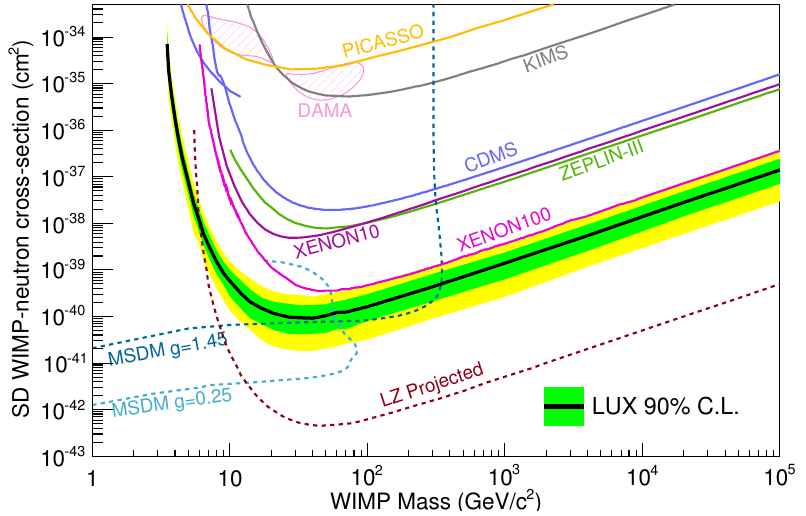
\includegraphics[scale=0.36]{LUX-SD-neutrons}
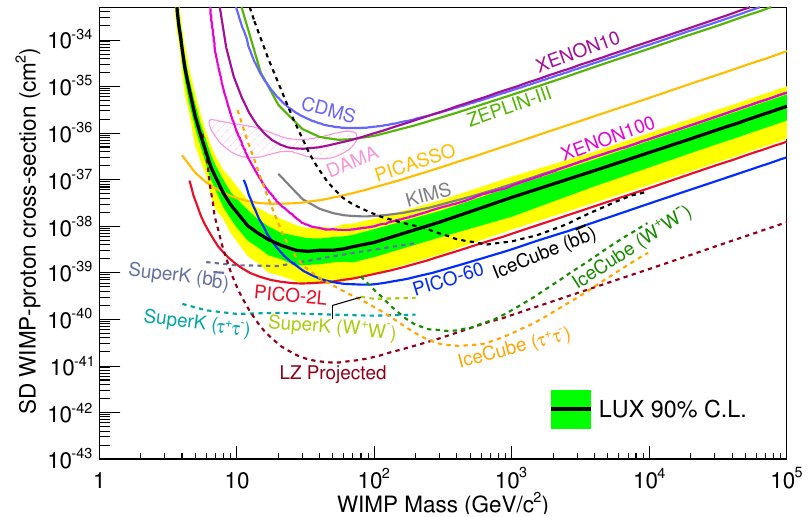
\includegraphics[scale=0.36]{LUX-SD-protons}
\end{center}
\caption{LUX upper limits on the WIMP-neutron (left) and -proton (right) elastic SD cross section at $90\%$ CL.
The Observed limit is shown in black with $\pm 1\sigma \, (\pm 2\sigma)$ band in green (yellow). Also, are shown the results from others experiments 
and the projected sensitivity for the LZ experiment. Taken from~\cite{Akerib:2016lao}. }
\label{fig:LUX-SD-2016}
\end{figure}
%
\begin{figure}[h]
\begin{center}
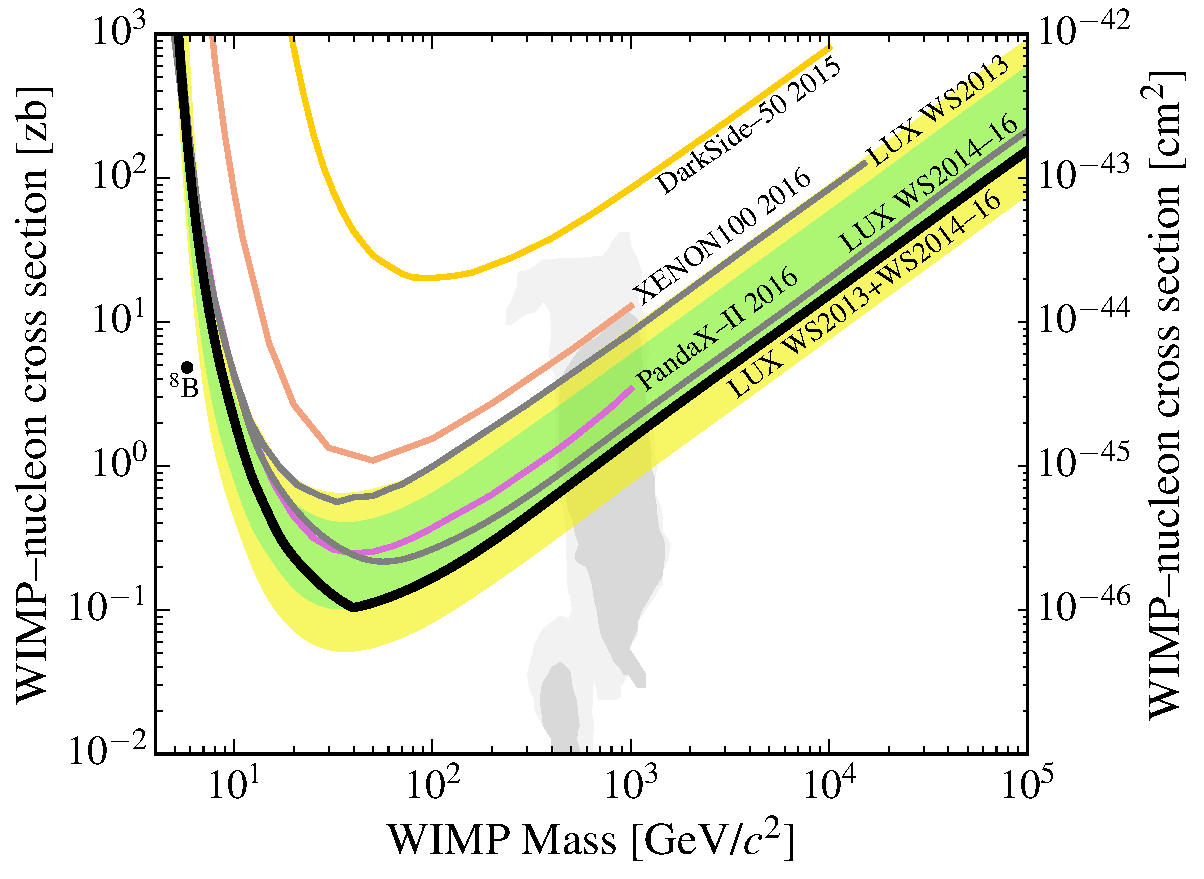
\includegraphics[width=10 cm,height=7 cm]{LUX-SI-2016}
\end{center}
\caption{LUX upper limits on the spin-independent elastic WIMP-nucleon
cross section at $90\%$ CL~\cite{Akerib:2016vxi}. }
\label{fig:LUX-SI-2016}
\end{figure}
%
The upper limits put strong constraints for all the DM theories based on the WIMP paradigm (Weakly Interacting Massive Particles). Specifically, all the region above the black line is excluded at $90\%$ CL.

\item \textbf{Indirect detection:}

Stable DM particles in the Universe could annihilate and produce a flux of gamma-rays, cosmic rays, neutrinos and anti-matter which can appear as an excess over the expected background, which is created by astrophysical features. In general, this flux can be written as
%
\begin{equation}
\underbrace{\frac{d\Phi}{d\Omega dE}}_{\text{Diff. Flux}} =  \frac{ \overbrace{\langle\sigma v \rangle}^{\text{Anni.\, Cross\, Section}}}{8\pi m_{\chi}^2} \times \underbrace{\frac{dN}{dE}}_{\text{Energy\, Spectrum}} \times \int_{\text{l.o.s}} ds \underbrace{\rho^2 (\overrightarrow{r}(s,\Omega))}_{\text{Dark\, Matter\, Distribution}},
\label{eq:flux}
\end{equation}
%
where $\Omega$ is the solid angle of the region of interest, $dN/dE$ is the energy spectrum (e.g. the number of particles produced per annihilation), $\sigma v$ is the annihilation cross section, and $\rho (\overrightarrow{r}(s,\Omega))$ is the DM density which should be integrated over the line of sight (l.o.s) from the observer to the source. This density is described by a specific profile, for instance, those shown in Table~\ref{table:DM-profiles}, where $\rho_{\odot}=0.3\, \text{GeV}/\text{cm}^3$ is the DM density at the sun, $r_s=20$~kpc is the scale radius of the halo and $R_{\odot}=8.5$~kpc is the distance from the sun to the center of the Galaxy~\cite{belanger2014micromegas}.
%
\begin{table}[h]
\centering
\begin{tabular}{|c|c|c|}\hline
Profile's name & Profile & \\\hline\hline
 & & \\
Zhao & $\rho(r) = \rho_{\odot} \left(\dfrac{R_{\odot}}{r}\right)^{\gamma} \left(\dfrac{r_s^{\alpha}+R_{\odot}^{\alpha}}{r_s^{\alpha}+r^{\alpha}}\right)^{\dfrac{\beta-\gamma}{\alpha}}$ & $\alpha=1$ \,, $\beta=3$ \,, $\gamma=1$ \\
 (in micrOMEGAS~\cite{belanger2014micromegas}) & &  \\\hline
 &  & \\
 Navarro-Frenk-White & $\rho(r) = \rho_{\odot}\, \frac{r_s}{r[1+ r/r_s]^2}$ & $\alpha=0.17$\\
 & & \\\hline
 &  & \\
Einasto profile & $\rho(r) = \rho_{\odot} \, exp \left[ -\frac{2}{\alpha} \left(\,  \left(\dfrac{r}{R_{\odot}}\right)^{\alpha}-1 \right) \right]$ &   $\alpha=0.17$ \\
 & & \\\hline
\end{tabular}
\caption{Mass density profiles for the dark matter in the Galaxy.}
\label{table:DM-profiles}
\end{table}

Several experiments for indirect detection of DM have been constructed. One of them is the \textit{Fermi} Large Area Telescope (\textit{Fermi}-LAT) which has a particle detector on board the Fermi gamma-ray space telescope spacecraft launched in 2008~\footnote{\url{http://fermi.gsfc.nasa.gov/}}. 
%
The searches of this experiment are focused in numerous exotic and beautiful phenomena, which can generate a lot of energy. For instance, Supermassive black holes, merging neutron stars, streams of hot gas moving close to the speed of light, etc. 
These are some of the marvels that generate gamma-ray radiation and the telescope is prepared to see it.
%
One of the searches has been concentrated in the dwarf spheroidal satellite galaxies (dSphs) of the Milky Way Galaxy, which are one of the most DM dominated objects known. 
In general, the \textit{Fermi}-LAT measures the flux of gamma-rays and reconstructs the signal as an interpretation of DM annihilation. 
Until now, the satellite has not seen a DM signal. 
However, it has presented upper limits on the thermal velocity averaged annihilation cross section $\langle \sigma v \rangle$ using some combined analysis~\cite{Ackermann:2015zua}. 
One of the principal results for DM self-annihilation are based on the photons created by the hadronization of the quarks, for instance, after the process $\text{DM DM} \to q\bar{q}$. 
The previous fact gives us a strong constraint in the $\langle \sigma v \rangle$ and will play an important roll in some of the analysis in this thesis.
 
%CONNECTION
Regarding indirect detection of dark matter, there is currently a puzzle related to the observation of an excess of gamma-ray with the \textit{Fermi}-LAT satellite that is one of the topics addressed in this thesis and for that reason will be briefly described in the next section.

\end{itemize}











%%%%%%%%%%%%%%%%%%%%%%%%%%%%%%%%%%%%%%%%%%%%%%%%%%%%%%%%%%%%%%%%%%%%%
\section{Dark matter interpretation of the galactic center excess}
\label{sec:intro-gce}
%
%TEXTO AMPLIADO DEL PAPER... MUCHOS PARRAFOS SON COPIADOS LITERALMENTE
WIMP particles appear effortlessly in many extensions of the SM that resolve outstanding theoretical and phenomenological problems which are not necessarily related to the DM puzzle.
 In some of these models, WIMPs can be produced in high energy colliders (collider DM searches), in elastic scatter with nucleons (direct DM searches) or in the annihilation and production of observable particles in astrophysical environments (indirect DM searches).
 High-energy photons in the gamma-ray ($\gamma$-ray) frequency constitute the most notable search channel of the latter category because they can travel almost unperturbed from their sources to the detectors.
 The Large Area Telescope on board the \textit{Fermi} satellite (\textit{Fermi}-LAT)~\cite{Fermi} is the most sensitive $\gamma$-ray detector in the range from 20 MeV to 300 GeV~\cite{Ackermann:2015zua}.

At the bottom of the gravitational well of the Milky Way Galaxy, the Galactic Center (GC) is expected to be the region displaying the brightest emission of DM annihilations in the $\gamma$-ray sky~\cite{Funk:review}.
However, there are multitude of non-thermal astrophysical sources in that region that complicate the identification of a tentative DM signal~\cite{Funk:review}. Observations of the inner few degrees around the GC with the \textit{Fermi}-LAT have revealed an excess of $\gamma$-rays ~\cite{Goodenough2009gk,Vitale:2009hr,Hooper:2010mq,hooper,AbazajianKaplinghat2012,AbazajianKaplinghat2013,GordonMacias2013}. 
The spectrum of the Galactic Center excess (GCE) peaks at about 1-3 GeV and its spatial morphology is spherically symmetric varying with radius $r$ around the GC as $r^{-2\gamma}$ with  $\gamma\sim 1.2$ which is clearly compatible with the DM density profile. 
This emission has been found to extend out in Galactic latitude ($b$) up to about $|b|\lesssim 20^\circ$ ~\cite{hooperslatyer2013,Daylan:2014,CaloreCholisWeniger2015,TheFermi-LAT:2015kwa} and its presence appears  to be robust with respect to systematic uncertainties~\cite{GordonMacias2013,MaciasGordon2014,Daylan:2014,Zho2015,CaloreCholisWeniger2015,PorterMurgia2015,TheFermi-LAT:2015kwa}.

Fig.~\ref{fig:GCE-less2} shows the GCE observed for $|b|<2^{\circ}$ and Galactic longitude $|l|<2^{\circ}$. 
This is the remaining excess after subtracting the Gamma Diffuse Emission of gamma rays (GDE) produced by cosmic rays that generate pions $\pi^0$ in collisions with the interstellar gas that latter decay and produce photons, by cosmic electrons which produce photons by bremsstrahlung emission and by photons accelerated by Inverse Compton scattering (ICS).
Fig.~\ref{fig:GCE-bigger2} shows the complete signal observed of the Galaxy for   $|b|>2^{\circ}$ and the remaining GCE after cleaning the map using the best GDE models. 

\begin{figure}[h]
\begin{center}
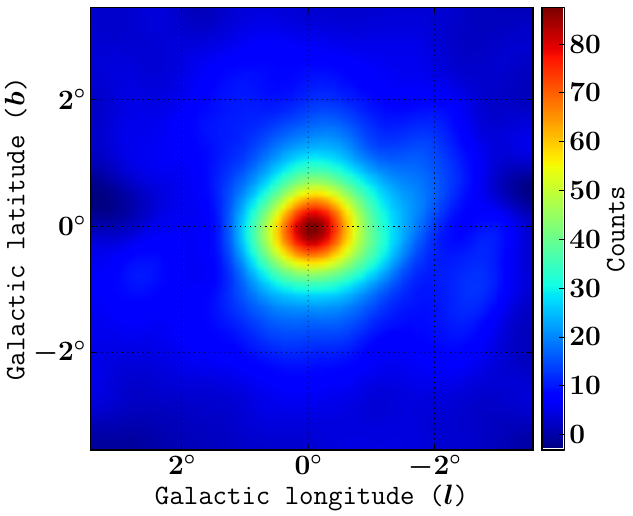
\includegraphics[scale=0.4]{latitude-less2}
\end{center}
\caption{Residual map or GCE signal for $|b,l|<2^{\circ}$. The counts were summed over the energy range 
$300$ MeV-$10$ GeV. The map spans a $7^{\circ}\times 7^{\circ}$ region of the sky centred in the Sgr A$^*$ position with a pixel size of $0.1^{\circ}\times 0.1^{\circ}$. Taken from~\cite{GordonMacias2013}.}
\label{fig:GCE-less2}
\end{figure}
%
\begin{figure}[h]
\begin{center}
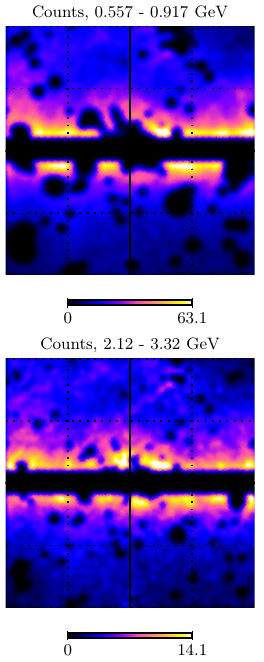
\includegraphics[scale=0.6]{latitude-bigger2a}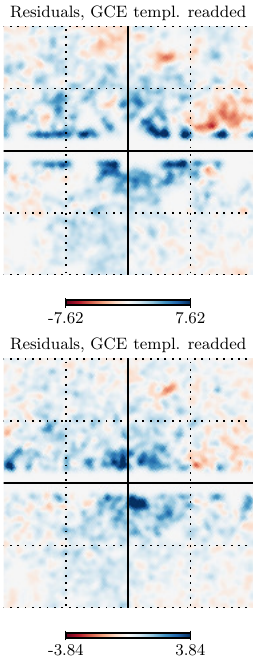
\includegraphics[scale=0.6]{latitude-bigger2b}
\end{center}
\caption{\textit{Left panels}: Counts map a various energies, with the disk cut $|b|>2^{\circ}$. \textit{Right panels}: Residual after sustracting the best Gamma Difuse emition model (GDE). Taken from~\cite{CaloreCholisWeniger2015}.}
\label{fig:GCE-bigger2}
\end{figure} 

There is an ongoing and intense debate as to what the origin of this signal is. A tentative explanation is an unresolved population of $\sim 1000$ millisecond pulsars (MSPs)~\cite{Abazajian:2010zy,AbazajianKaplinghat2012,Wharton2012,GordonMacias2013,GordonMacias2013erratum,Mirabal2013,MaciasGordon2014,YuanZhang2014,BrandtKocsis2015,Lacroix:2015wfx,O'Leary:2016osi} or young pulsars \cite{OLeary2015,O'Leary:2016osi}.
 Nevertheless, some studies~\cite{Hooper2013,CholisHooperLinden2015,PetrovicSerpicoZaharijas2015,Lee2015,BartelsKrishnamurthyWeniger2015,Linden2015} have pointed out about the difficulties of reconciling this hypothesis with the GCE extending out as far as $\sim 10^\circ$ from the GC. On the other hand, recent works claim that the GCE is not smooth~\cite{Lee:2015fea,Bartels:2015aea}, and if confirmed, this would lend support to the MSPs alternative.
 Another scenario put forward is a series of energetic cosmic-ray injections in the GC \cite{CarlsonProfumo,Petrovic2014}.
 However, if the injected particles are mainly protons, it has been shown~\cite{MacGorCroProf2015} that this scenario is incompatible with the spatial morphology of the GCE in the inner $\sim 2^\circ$ of the Galaxy.
 In case the burst events contain protons as well as leptons, Ref~\cite{Cholis2015} finds suitable models that appear fine-tuned.

Despite these astrophysical uncertainties, a DM interpretation of the GCE cannot be ruled out yet~\cite{Goodenough2009gk,Hooper:2010mq,hooper,AbazajianKaplinghat2012,AbazajianKaplinghat2013,GordonMacias2013,MaciasGordon2014,Abazajian2014,Daylan:2014,Lacroix:2015wfx}.
   In this context, the spatial morphology of the GCE can be accommodated with a Navarro-Frenk-White (NFW) profile with a mildly contracted cusp of $\gamma\sim 1.2$, the measured spectrum implies a WIMP mass in the GeV energy range and an interaction cross section that coincides with the thermal relic cross section. 

A recent study of the GCE~\cite{CaloreCholisWeniger2015} selected a target region ($|b|>2^\circ$) that excluded the core of the GC. Additionally, the systematic uncertainties in the Galactic diffuse emission were estimated in a manner that made the low and high energy tails of the spectrum more uncertain than in previous analyses~\cite{GordonMacias2013,MaciasGordon2014,Abazajian2014,Daylan:2014}, which focused on a smaller region containing the inner $\sim 2^\circ$ of the GC. Although it is possible that the greater degree of uncertainty in the tails found by~\cite{CaloreCholisWeniger2015} is due to an intricate overlap of the GCE with the Fermi Bubbles~\cite{suslatyerfinkbeiner2010,Fermi-LAT:AnnaFranckowiak}, it is interesting that this uncertainty also allows much more freedom for DM models fitting the GCE~\cite{Logan:2010nw,Buckley:2010ve,Zhu:2011dz,Marshall:2011mm,Boucenna:2011hy,Buckley:2011mm,Anchordoqui:2013pta,Buckley:2013sca,Hagiwara:2013qya,Okada:2013bna,Huang:2013apa,Modak:2013jya,Boehm:2014hva,Alves:2014yha,Berlin:2014tja,Agrawal:2014una,Izaguirre:2014vva,Cerdeno:2014cda,Ipek:2014gua,Boehm:2014bia,Ko:2014gha,Abdullah:2014lla,Ghosh:2014pwa,Martin:2014sxa,Basak:2014sza,Berlin:2014pya,Cline:2014dwa,Han:2014nba,Detmold:2014qqa,Wang:2014elb,Chang:2014lxa,Arina:2014yna,Cheung:2014lqa,McDermott:2014rqa,Huang:2014cla,Balazs:2014jla,Ko:2014loa,Okada:2014usa,Ghorbani:2014qpa,Banik:2014eda,Borah:2014ska,Cahill-Rowley:2014ora,Guo:2014gra,Freytsis:2014sua,Heikinheimo:2014xza,Arcadi:2014lta,Richard:2014vfa,Cao:2014efa,Bell:2014xta,Cerdeno:2015ega,Caron:2015wda,Bertoneetal,Freeseetal}.  


Significant effort has been made in exploring the properties of DM models that can explain the GCE while being consistent with other indirect, direct and collider constraints~\cite{Logan:2010nw,Buckley:2010ve,Zhu:2011dz,Marshall:2011mm,Boucenna:2011hy,Buckley:2011mm,Anchordoqui:2013pta,Buckley:2013sca,Hagiwara:2013qya,Okada:2013bna,Huang:2013apa,Modak:2013jya,Boehm:2014hva,Alves:2014yha,Berlin:2014tja,Agrawal:2014una,Izaguirre:2014vva,Cerdeno:2014cda,Ipek:2014gua,Boehm:2014bia,Ko:2014gha,Abdullah:2014lla,Ghosh:2014pwa,Martin:2014sxa,Basak:2014sza,Berlin:2014pya,Cline:2014dwa,Han:2014nba,Detmold:2014qqa,Wang:2014elb,Chang:2014lxa,Arina:2014yna,Cheung:2014lqa,McDermott:2014rqa,Huang:2014cla,Balazs:2014jla,Ko:2014loa,Okada:2014usa,Ghorbani:2014qpa,Banik:2014eda,Borah:2014ska,Cahill-Rowley:2014ora,Guo:2014gra,Freytsis:2014sua,Heikinheimo:2014xza,Arcadi:2014lta,Richard:2014vfa,Cao:2014efa,Bell:2014xta,Cerdeno:2015ega,Caron:2015wda,Bertoneetal,Freeseetal}.
 Of great interest are the properties of minimal supersymmetric extensions of the SM (MSSM)~\cite{Cheung:2014lqa,Cahill-Rowley:2014ora,Cao:2014efa,Cerdeno:2015ega,Caron:2015wda,Bertoneetal,Freeseetal} that can fit the GCE.
 When these extensions are studied in light of the GCE extracted from the region $|b|>2^\circ$ of the GC, the required neutralino annihilation rates to mainly the $W^+W^-$ and $\bar{t}t$ channels are found to comply with the LEP or LHC bounds on sfermion masses.
However, we do not restrict ourselves to supersymmetric models. Instead, we take the approach of studying a simplified DM model in which the DM candidate is a mixture, generated by the interaction with the Higgs boson, of a SM fermion singlet and the neutral components of an electroweak doublet vector-like fermion~\cite{ArkaniHamed:2005yv,Mahbubani:2005pt,D'Eramo:2007ga,Enberg:2007rp}. This model, also known as the singlet$-$doublet fermion DM (SDFDM) model, is one of the simplest UV realizations of the fermion Higgs portal ~\cite{Patt:2006fw} with the SM Higgs boson as the mediator between the visible and dark sectors. In fact, the dark sector of the SDFDM model (along with the stabilizing discrete symmetry) is part of the minimal setup expected when the SM is extended by new physics which is to some extent related to lepton and baryon number conservation~\cite{Arbelaez:2015ila,Arkani-Hamed:2015vfh}. While being free of many theoretical biases, this  model allows us to extract maximal phenomenological information from a framework that is a good representation of the WIMP paradigm \cite{ArkaniHamed:2005yv,Mahbubani:2005pt,D'Eramo:2007ga,Enberg:2007rp,Cohen:2011ec,Cheung:2013dua,Abe:2014gua,Calibbi:2015nha,Freitas:2015hsa,Abdallah:2015ter}.%\footnote{ If scalar singlets are added to its particle content, neutrino masses can also be radiatively generated in this generic class of models~\cite{Restrepo:2015ura}.}.     
Accordingly, the SDFDM model is set to become one of the models to be implemented in future searches for DM particles at the LHC \cite{Abdallah:2015ter} and a future 100 TeV hadron collider \cite{Gori:2014oua,Arkani-Hamed:2015vfh}.  

To understand how neutrino masses will be incorporated in a SDFDM model, it is important to explain briefly the relation between the dark matter and neutrino masses, more specifically, how to generated neutrino masses from a dark sector. This relation will be described in the next section.











%%%%%%%%%%%%%%%%%%%%%%%%%%%%%%%%%%%%%%%%%%%%%%%%%%%%%%%%%%%%%%%%%%%%%
\section{Relations between dark matter and the non-zero neutrino masses}

\subsection*{Neutrino physics in a nutshell}
\label{sec:intro-neutrino}
%
Although, neutrinos in the SM are massless, current neutrino oscillation data had established the non-zero value of neutrino masses, which is a clear indication of new physics beyond the SM. 
These neutrino data can be described within the framework of a $3\times 3$ mixing matrix $U$ between the flavor eigenstates $\nu_l=(\nu_e,\nu_{\mu},\nu_{\tau})$ and the mass eigenstates $\nu_i=(\nu_1,\nu_2,\nu_3)$, such that
%
\begin{align}
|\nu_l\rangle = \sum_i U_{li}^*|\nu_i\rangle \,.
\end{align}
%
In the case of Dirac neutrinos, the mixing matrix  $U$ depends on three mixing angles $\theta_{12}$, $\theta_{13}$, $\theta_{23}$ and one CP-violating phase $\delta$, while in the case of Majorana neutrinos there are two additional phases~\cite{Akhmedov:1999uz}. 
In general, it is convenient to use the parametrization that coincides with the quark mixing matrix given by
%
\begin{displaymath}
U=\left(\begin{array}{c c c}
c_{12}c_{13} & s_{12}c_{13}& s_{13}e^{-i\delta}\\
-s_{12}c_{23}-c_{12}s_{23}s_{13}e^{i\delta} & c_{12}c_{23}-s_{12}s_{23}s_{13}e^{i\delta} & s_{23}c_{13}\\
s_{12}s_{23}-c_{12}c_{23}s_{13}e^{i\delta} & -c_{12}s_{23}-s_{12}c_{23}s_{13}e^{i\delta} & c_{23}c_{13}
\end{array} \right)\,,
\end{displaymath}
%
where $c_{ij}=\cos \theta_{ij}$ and $s_{ij}=\sin \theta_{ij}$.

In the neutrino oscillation theory, the probability of the transformation of a flavor eigenstates neutrino $\nu_{a}$ into another one $\nu_{b}$ in a time $t$ is given by~\cite{Akhmedov:1999uz}
%
\begin{align}
P(\nu_a \to \nu_b; t)=|U_{bj}e^{-iE_j t}U_{aj}^*|^2\,,
\end{align}
%
where the energy $E_i$ and the momenta $p$ for the eigenstate of mass $m_i$ are related by
\begin{align}
E_i=\sqrt{p^2+m_i^2}\approx p+\dfrac{m_i^2}{2p}\,.
\end{align}
%
There are some important limit cases in which this probability is computed. For instance, when the neutrino mass squared differences $\Delta m_{ij}^2=m_i^2-m_j^2$ have a hierarchy
%
\begin{align}
|\Delta m_{21}^2| \ll |\Delta m_{31}^2| \simeq |\Delta m_{32}^2|
\Rightarrow
\left\{
\begin{array}{ll}
 m_1 \ll (\lesssim)\, m_2 \ll m_3 & \text{ Normal hierarchy NH } \\
 m_3 \ll m_1 \approx m_2 & \text{ Inverted  hierarchy IH }\,.
\end{array}
\right. 
\end{align}
%
These hierarchies are good motivated by the fact that the solar neutrino data indicates $\Delta m_{21}^2 =\Delta m_{\odot}^2 \sim 10^{-5}$ eV$^2$ for the solution of the solar neutrino problem through the matter neutrino oscillations ($\Delta m_{\odot}^2 \sim 10^{-10}$ eV$^2$ through the vacuum oscillations).  Whereas the explanation of the atmospheric neutrino oscillations experiments requires $\Delta m_{32}^2 =\Delta m_{\text{atm}}^2 \sim 10^{-3}$ eV$^2$ much larger than  $\Delta m_{\odot}^2$. For a complete list of neutrino oscillation parameters see Table~\ref{tab:neutrino-parameters}.

\begin{table}[h]\centering
   \begin{tabular}{lccc}
    \hline
    parameter & best fit $\pm$ $1\sigma$ &  2$\sigma$ range& 3$\sigma$ range
    \\
    \hline
    $\Delta m^2_{21}\: [10^{-5}\eVq]$
    & 7.60$^{+0.19}_{-0.18}$  & 7.26--7.99 & 7.11--8.18 \\[3mm] 
    %%
    $|\Delta m^2_{31}|\: [10^{-3}\eVq]$ (NH)
    &  2.48$^{+0.05}_{-0.07}$ &  2.35--2.59 &  2.30--2.65\\
    $|\Delta m^2_{31}|\: [10^{-3}\eVq]$ (IH)
    &  2.38$^{+0.05}_{-0.06}$ &  2.26--2.48 &  2.20--2.54 \\[3mm] 
    %%	
    $\sin^2\theta_{12} / 10^{-1}$
    & 3.23$\pm$0.16 & 2.92--3.57 & 2.78--3.75\\
    $\theta_{12}$ 
    & 34.6$\pm$1.0 & 32.7--36.7 & 31.8--37.8\\[3mm]  
    %%
    $\sin^2\theta_{23} / 10^{-1}$ (NH)
    &	5.67$^{+0.32}_{-1.28}$ 
    & 4.13--6.23 & 3.92 -- 6.43 \\
    $\theta_{23}$ %(NH)
    & 48.9$^{+1.9}_{-7.4}$ & 40.0--52.1 & 38.8--53.3 \\ 
    $\sin^2\theta_{23} / 10^{-1}$ (IH)
    & 5.73$^{+0.25}_{-0.43}$ & 4.32--6.21 & 4.03--6.40 \\
    $\theta_{23}$ %(IH)
    & 49.2$^{+1.5}_{-2.5}$ & 41.1--52.0 & 39.4--53.1\\[3mm]  
    %%	
    $\sin^2\theta_{13} / 10^{-2}$ (NH)
    & 2.34$\pm$0.20 & 1.95--2.74 & 1.77--2.94 \\
    $\theta_{13}$ %(NH)
    &	8.8$\pm$0.4 & 8.0--9.5 & 7.7--9.9\\
    $\sin^2\theta_{13} / 10^{-2}$ (IH)
    & 2.40$\pm$0.19 & 2.02--2.78 & 1.83--2.97 \\
     $\theta_{13}$ %(IH)
     & 8.9$\pm$0.4 & 8.2--9.6 & 7.8--9.9\\[3mm]
    %%	
   $\delta/\pi$ (NH)
   	& 1.34$^{+0.64}_{-0.38}$ & 0.0--2.0 & 0.0--2.0 \\
   $\delta/\pi$ (IH)	
   	& 1.48$^{+0.34}_{-0.32}$ & 0.0--0.14 \& 0.81-2.0 & 0.0--2.0 \\	
       \hline
     \end{tabular}
     \caption{ \label{tab:summary} Neutrino oscillation parameters
       summary taken from~\cite{Forero:2014bxa}. For $\Delta m^2_{31}$, $\sin^2\theta_{23}$, $\sin^2\theta_{13}$, 
       and $\delta$ the upper (lower) row corresponds to normal (inverted)
       neutrino mass hierarchy.}
\label{tab:neutrino-parameters}
\end{table}











\subsection*{How to generate neutrino masses from a dark sector?}
%
In this thesis, it is assumed that the neutrinos of the SM are Majorana particles.
In that case, their so small masses can be understood if there is a new physics beyond the SM as it will briefly describe in the present section. 
It have been shown that the lower operator which generates Majorana neutrino masses is the $d=5$ Weinberg operator~\cite{PhysRevLett.43.1566}
%
\begin{align}
\label{eq:weinberg-operator}
\mathcal{L}=\dfrac{1}{2}c_{\alpha\beta}^{d=5} \,\, \left(\overline{L_{\alpha}^c}\widetilde{H}^*\right) \left( \widetilde{H}^{\dagger}L_{\beta}\right) + \text{h.c.}  \,,
\end{align}
%
where $H=\left(H^+,H^0\right)^T$ is the Higgs doublet, $\widetilde{H}=i\sigma_2 H^*$,  $L_{\alpha}=\left(\nu_{\alpha L},e_{\alpha L}\right)^T$ are the left-handed lepton doublets of the SM with $\alpha$ the flavor number and $c_{\alpha\beta}^{d=5}\propto 1/\Lambda $ is a model dependent coefficient that characterize the scale of the new physics.  
All the models where the neutrinos are Majorana particles are reduced to this operator or a higher dimensional equivalent $(d > 5)$ when the new physics is integrated out~\cite{Bonnet:2012kz}.

At tree level, there are three ways to generate this operator. These are known as type-I, type-II and type-III see-saw mechanisms when the mediator is a singlet fermion $N$, a triplet scalar $\Delta$ or a triplet fermion $\Sigma$ respectively. These three cases are schematically shown in Fig.~\ref{fig:see-saw-tree-level}.
%
\begin{figure}[h]
\begin{center}
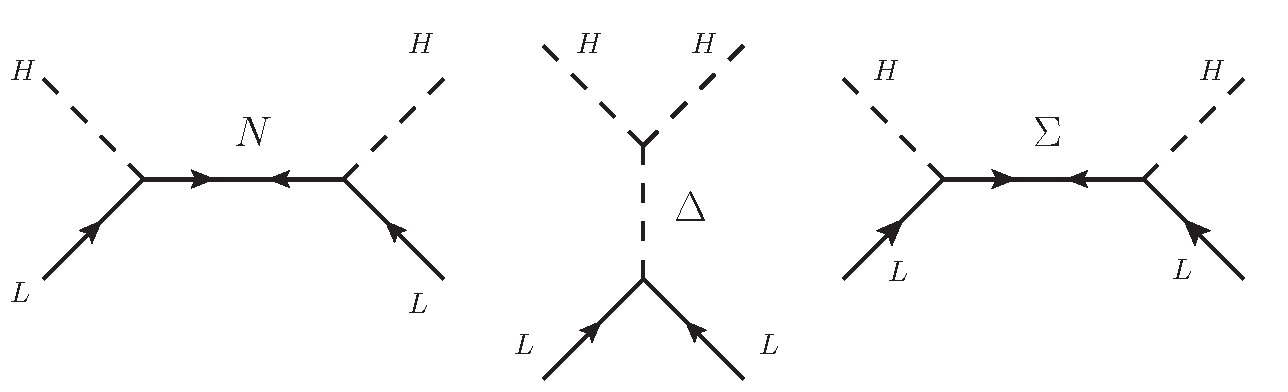
\includegraphics[scale=0.7]{fig4.pdf}
\end{center}
\caption{The three realizations of the see-saw mechanism at tree level.}
\label{fig:see-saw-tree-level}
\end{figure} 

From Eq.~\eqref{eq:weinberg-operator} we can see that the neutrino mass scale is roughly given by $m_{\nu_{\alpha}}\propto \langle H^0\rangle^2/\Lambda$,  where $\langle H^0\rangle$ is the vacuum expectation value of the SM Higgs boson. Notice that in order to have small neutrino masses the $\Lambda$ points to the scale of a grand unified theory (GUT).  
%Therefore, in these see-saw models the new physics scale will be impossible to test at the LHC.

On the other hand, at one-loop level, when the neutrino masses are generated radiatively, 
one additional suppression comes from the loop.
In this case, the new physics and consequently the dark sector could be at the electroweak scale (EW) and the mechanism could be tested with the current direct, indirect and colliders experiments.
%
\begin{figure}[h]
\begin{center}
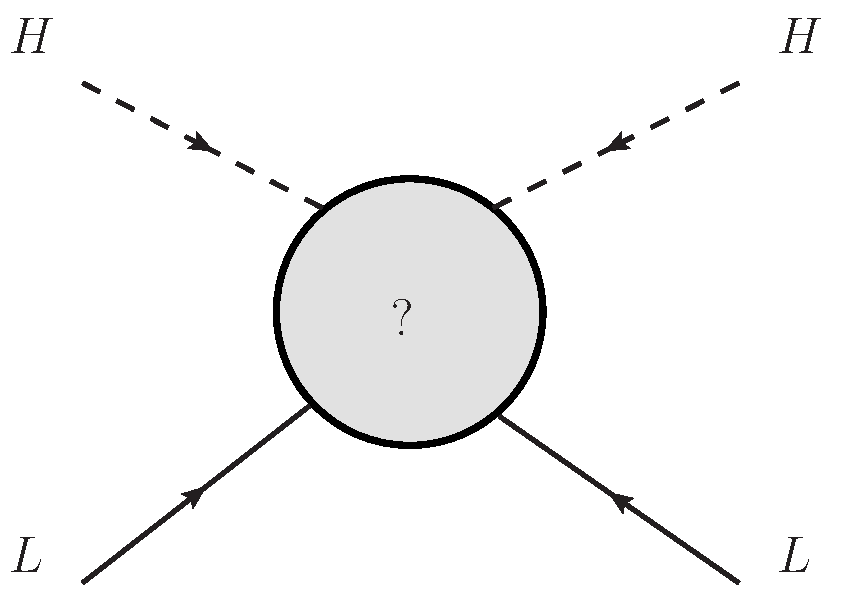
\includegraphics[scale=0.4]{fig5.pdf}
\end{center}
\caption{Schematic realization of the radiative see-saw mechanism at one-loop level. The new dark sector and consequently the DM particle is circling in the loop.}
\label{fig:see-saw-one-loop}
\end{figure} 
%
This realization of the $d=5$ Weinberg operator is diagrammatically shown in Fig.~\ref{fig:see-saw-one-loop}. 
For a complete diagrammatically and systematic study of the $d=5$ Weinberg operator at one-loop level see the Ref.~\cite{Bonnet:2012kz}.  
In particular, in this thesis, one specific realization of a well-motivated DM model is studied which will be described in the next chapter.

As a final comment and motivation, it is important to keep in mind that at one-loop level, the neutrino masses are approximately given by 
%
\begin{align}
m_{\nu}\propto 
\dfrac{\langle H^0\rangle ^2 }{\Lambda} \times \left(\dfrac{\epsilon}{16\pi^2}\right) \,,
\end{align}
%
where $\epsilon$ expresses symbolically the loop suppression. 
Therefore, the small neutrino masses are explained by the loop suppression and by the scale of the new physics.  See, for example, the see-saw radiative model described in~\cite{Ma:2006km}.


